\documentclass[]{article}
\usepackage{lmodern}
\usepackage{amssymb,amsmath}
\usepackage{ifxetex,ifluatex}
\usepackage{fixltx2e} % provides \textsubscript
\ifnum 0\ifxetex 1\fi\ifluatex 1\fi=0 % if pdftex
  \usepackage[T1]{fontenc}
  \usepackage[utf8]{inputenc}
\else % if luatex or xelatex
  \ifxetex
    \usepackage{mathspec}
  \else
    \usepackage{fontspec}
  \fi
  \defaultfontfeatures{Ligatures=TeX,Scale=MatchLowercase}
\fi
% use upquote if available, for straight quotes in verbatim environments
\IfFileExists{upquote.sty}{\usepackage{upquote}}{}
% use microtype if available
\IfFileExists{microtype.sty}{%
\usepackage{microtype}
\UseMicrotypeSet[protrusion]{basicmath} % disable protrusion for tt fonts
}{}
\usepackage[margin=1in]{geometry}
\usepackage{hyperref}
\hypersetup{unicode=true,
            pdftitle={In-flight Wifi Pricing Optimization},
            pdfauthor={California State University, Fullerton; In collaboration with Panasonic and Black Swan Data; Romain Drai, Tin Huynh, James Luo, Shan Jiang, Jessica Shin, Foon Wong, Tingting Xu},
            pdfborder={0 0 0},
            breaklinks=true}
\urlstyle{same}  % don't use monospace font for urls
\usepackage{longtable,booktabs}
\usepackage{graphicx,grffile}
\makeatletter
\def\maxwidth{\ifdim\Gin@nat@width>\linewidth\linewidth\else\Gin@nat@width\fi}
\def\maxheight{\ifdim\Gin@nat@height>\textheight\textheight\else\Gin@nat@height\fi}
\makeatother
% Scale images if necessary, so that they will not overflow the page
% margins by default, and it is still possible to overwrite the defaults
% using explicit options in \includegraphics[width, height, ...]{}
\setkeys{Gin}{width=\maxwidth,height=\maxheight,keepaspectratio}
\IfFileExists{parskip.sty}{%
\usepackage{parskip}
}{% else
\setlength{\parindent}{0pt}
\setlength{\parskip}{6pt plus 2pt minus 1pt}
}
\setlength{\emergencystretch}{3em}  % prevent overfull lines
\providecommand{\tightlist}{%
  \setlength{\itemsep}{0pt}\setlength{\parskip}{0pt}}
\setcounter{secnumdepth}{0}
% Redefines (sub)paragraphs to behave more like sections
\ifx\paragraph\undefined\else
\let\oldparagraph\paragraph
\renewcommand{\paragraph}[1]{\oldparagraph{#1}\mbox{}}
\fi
\ifx\subparagraph\undefined\else
\let\oldsubparagraph\subparagraph
\renewcommand{\subparagraph}[1]{\oldsubparagraph{#1}\mbox{}}
\fi

%%% Use protect on footnotes to avoid problems with footnotes in titles
\let\rmarkdownfootnote\footnote%
\def\footnote{\protect\rmarkdownfootnote}

%%% Change title format to be more compact
\usepackage{titling}

% Create subtitle command for use in maketitle
\providecommand{\subtitle}[1]{
  \posttitle{
    \begin{center}\large#1\end{center}
    }
}

\setlength{\droptitle}{-2em}

  \title{In-flight Wifi Pricing Optimization}
    \pretitle{\vspace{\droptitle}\centering\huge}
  \posttitle{\par}
    \author{California State University, Fullerton \\ In collaboration with Panasonic and Black Swan Data \\ Romain Drai, Tin Huynh, James Luo, Shan Jiang, Jessica Shin, Foon Wong,
Tingting Xu}
    \preauthor{\centering\large\emph}
  \postauthor{\par}
      \predate{\centering\large\emph}
  \postdate{\par}
    \date{May 1, 2019}

\usepackage{titling}
\usepackage{float}
\floatplacement{figure}{H}
\pretitle{\begin{center}\LARGE
\includegraphics[width=2cm]{csuflogo.png}\\[\bigskipamount]}
\posttitle{\end{center}}
\usepackage{amsmath,amssymb}
\setlength{\columnsep}{18pt}

\begin{document}
\maketitle

\hypertarget{introduction}{%
\subsection{1. Introduction}\label{introduction}}

Dynamic pricing is a pricing policy in which a firm adjusts the price of
their product as a function of its perceived demand in order to maximize
profit. A common challenge when applying machine learning techniques for
pricing optimization is the lack of past observations. The specific
problem of inflight WiFi pricing optimization is no exception. While
Panasonic collects millions of transaction per year from its wide
network of partner airlines, the actual number pricing policies for
learning consumer behavior are much more limited if we consider
regional, product and hardware differences. Fortunately, if we
strategically generalize some of the variables, we can create
opportunities for learning.

From literature research, we choose to adopt a two-staged framework to
tackle this problem. First, a demand, or price-response model is built
to understand the effect of the different factors. Then, a dynamic
pricing model is built to find the optimal pricing. The appeal aspect of
this framework is that the problem is broken down into two independent
stages. For this project, we can build upon any prior work done on the
demand model; conversely, improvements to the demand model can be made
without changing the pricing solver. Finally, it provides an evaluation
scheme for validation and future improvements.

\hypertarget{data-description}{%
\subsection{2. Data Description}\label{data-description}}

The dataset we analyzed consists of 4.1 million distinct in-flight
internet sessions purchased by customers on airlines partnered with
Panasonic Avionics from November 2016 to November 2018. In table 1, the
number of unique sessions, flights, geographic factors are listed.

\begin{longtable}[]{@{}cc@{}}
\caption{Unqiue factors}\tabularnewline
\toprule
\endhead
\begin{minipage}[t]{0.29\columnwidth}\centering
\textbf{SessionID}\strut
\end{minipage} & \begin{minipage}[t]{0.13\columnwidth}\centering
4181197\strut
\end{minipage}\tabularnewline
\begin{minipage}[t]{0.29\columnwidth}\centering
\textbf{FlightID}\strut
\end{minipage} & \begin{minipage}[t]{0.13\columnwidth}\centering
567089\strut
\end{minipage}\tabularnewline
\begin{minipage}[t]{0.29\columnwidth}\centering
\textbf{UserID}\strut
\end{minipage} & \begin{minipage}[t]{0.13\columnwidth}\centering
1142383\strut
\end{minipage}\tabularnewline
\begin{minipage}[t]{0.29\columnwidth}\centering
\textbf{Routes}\strut
\end{minipage} & \begin{minipage}[t]{0.13\columnwidth}\centering
3048\strut
\end{minipage}\tabularnewline
\begin{minipage}[t]{0.29\columnwidth}\centering
\textbf{OriginIATA}\strut
\end{minipage} & \begin{minipage}[t]{0.13\columnwidth}\centering
452\strut
\end{minipage}\tabularnewline
\begin{minipage}[t]{0.29\columnwidth}\centering
\textbf{DestinationIATA}\strut
\end{minipage} & \begin{minipage}[t]{0.13\columnwidth}\centering
439\strut
\end{minipage}\tabularnewline
\begin{minipage}[t]{0.29\columnwidth}\centering
\textbf{Orig\_Country}\strut
\end{minipage} & \begin{minipage}[t]{0.13\columnwidth}\centering
137\strut
\end{minipage}\tabularnewline
\begin{minipage}[t]{0.29\columnwidth}\centering
\textbf{Dest\_Country}\strut
\end{minipage} & \begin{minipage}[t]{0.13\columnwidth}\centering
138\strut
\end{minipage}\tabularnewline
\begin{minipage}[t]{0.29\columnwidth}\centering
\textbf{Airline}\strut
\end{minipage} & \begin{minipage}[t]{0.13\columnwidth}\centering
23\strut
\end{minipage}\tabularnewline
\bottomrule
\end{longtable}

In addition to the factors above, the dataset also include information
such as number of passengers on flight, product pricing, product names,
aircraft type, entertainment options.

To understand the geographic distribution, a network graph of the wifi
sessions was generated in fig. 1. The node and edge weights were based
on the number of wifi sessions purchased. We can see that although there
were more than 3400 hundred routes, the majority of wifi sessions
associated with Panasonic partners were heavily concentrated in North
America and selected European cities.

The most crucial pieces of information would be the price paid and the
data consumption by the consumer, as these variable gave us a direct
link to the revenue and cost associated with providing in-flight wifi
services. Distribution of these two key variables are show in fig. 2,
with the top 0.5\% removed to avoid outliers. The distribution of the
price paid revealed one of the key data challenge to this project: the
lack of pricing variation. With 23 partner airlines, and roughly 3 to 5
unique products per flight route, the distribution of the pricing was
unevenly concentrated in a few particular price points between \$5 to
\$20 USD.

\begin{figure}
\centering
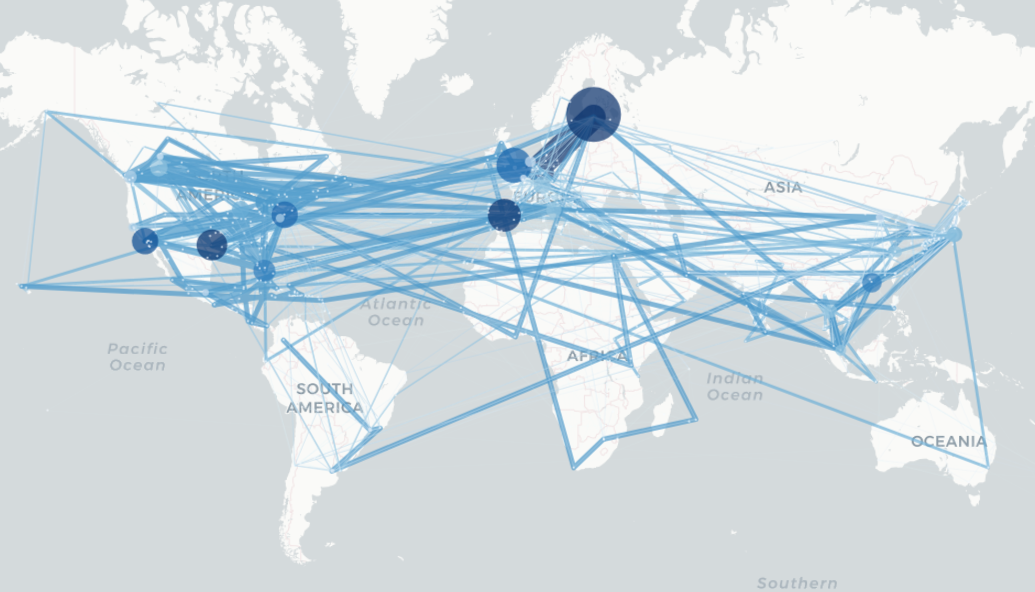
\includegraphics[width=6.25in,height=\textheight]{figures/flight_network.png}
\caption{Network graph of wifi sessions}
\end{figure}

\begin{figure}
\centering
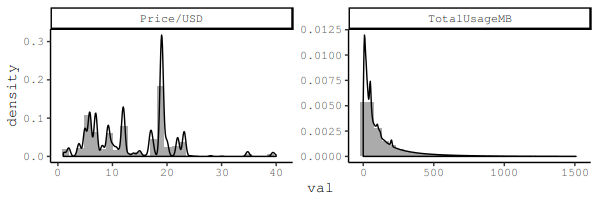
\includegraphics{figures/price_data_dist.png}
\caption{Distribution of price paid and data consumption}
\end{figure}

\pagebreak

\hypertarget{modeling-approach}{%
\subsection{3. Modeling approach}\label{modeling-approach}}

\hypertarget{demand-model}{%
\paragraph{Demand model}\label{demand-model}}

We have found a wide variety of demand model specifications. Parametric
models from the generalized linear model family are well studied and
their success depends on whether their assumptions are met. In addition,
their gradient are relatively easy to obtain, allowing optimising
problems to be solved. On the other hand, powerful machine learning
techniques such as random forest or neural networks can also be
employed, but additional optimization problem can become challenging.

The goal for the demand model is to capture the most important factors
that influence demand.

\[
    Q_t = \psi_t (P_1, P_2, ..., P_N),
\]

here \(Q\) is the total sales and \(\psi(.)\) is the demand function at
time \(t\). \(\psi(.)\) can take on any functional form.

Previously, Panasonic data science team have built a successful demand
model based on random forest. They have found that the take rate/sales
per flight for their products depend greatly on covariates such as the
number of passengers, flight route, red-eye, etc. To estimate demand
difference, for example between regular vs red-eye flights, we can check
model prediction by holding other factors constant.

\hypertarget{common-pricing-optimization-model}{%
\paragraph{Common pricing optimization
model}\label{common-pricing-optimization-model}}

While a demand model can provide prediction on demand and easily solve
for pricing that maximizes revenue, total profit needs to be separately
calculated. When cost is unrelated to the covariates that drive the
demand model, the optimization problem can be formulated as:

\[
    \underset{P_1,\dots,P_N}{\max}   \Pi = \sum_{i=1}^N [\psi_t (P_1, P_2, \dots, P_N)(P_t - C_t)]
\] where \(\Pi\) is the total profit across a planning horizon, as a
function of a et of pricing \(P_1, \dots, P_N\), and average price and
cost \(P_t\), \(C_t\).

This is a common approach to a dynamic pricing optimzation problem and
one that we initially considered.

Early in our research process, we proposed to use evolutionary
algorithms (EA) to optimize the model above. However, because our model
now needs to predict demand both in the form of purchases and data
consumption simultaneously, we adjusted our approach, and combine the
two directly into a single profit feature.

\hypertarget{final-approach}{%
\paragraph{Final approach}\label{final-approach}}

Because data usage spanned such a wide range, we must incoporate cost
into modeling consideration and the optimization problem needs to be
adjusted.

For cost estimation, we will assume a linear relationship between
customer data usage and true cost. This functional relationship base on
actual business situation and can be included as a functional parameter.
In addition, capacity and pricing limiting constraints can be imposed.
In figure 2, we can see that the data usage distribution was smooth and
concentrated around 100MB per session.

Therefore, our goal became: \[
     \underset{P_1,\dots,P_N}{\max}   G_t = \psi_t (P_1, P_2, ..., P_N),  \qquad \text{for all P's}
\]

here \(G\) is the gross profit and \(\psi(.)\) is a demand function at
time \(t\). \(\psi(.)\) can take on any functional form.

Finally, to generate recommendation for pricing, we then use grid search
to find the best pricing at a few fixed product specifications.

\hypertarget{data-preparation}{%
\subsection{4. Data preparation}\label{data-preparation}}

\hypertarget{predictive-model-target}{%
\paragraph{Predictive model target}\label{predictive-model-target}}

The dataset provided us pricing and usage data at the user level. With a
constant per-megabyte cost of data, we are able to calculate the
profit-per-session of each session of data usage.

To also capture the demand in our model target, we must also calculate
the amount of purchases. We decided to approach this at a flight level.
Using the estimated figure for total passengers on each flight, we
calculate the rate of profit as:

\[
\text{profit per person} = \frac{\text{total revenue} - \text{total cost} }{\text{total passengers}}
\]

\begin{figure}
\centering
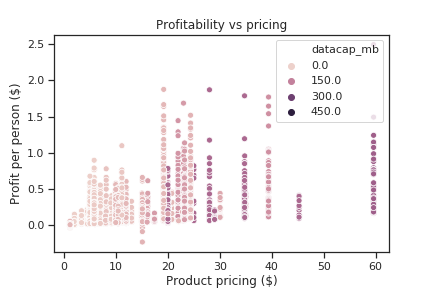
\includegraphics[width=\textwidth,height=2.60417in]{figures/profit_scatter.png}
\caption{Distribution of profit}
\end{figure}

\hypertarget{feature-engineering}{%
\paragraph{Feature engineering}\label{feature-engineering}}

A piece of information that we found to have significant effect on model
result is the data and time allowance. By extracting the numerical
values from the product name, we gained two powerful features that would
prove to improve model performance greatly.

Tables 2 and 3 below show examples of the feature extraction and the
number of products that have the relevant information.

\begin{longtable}[]{@{}ccc@{}}
\caption{Example of feature extraction from product name}\tabularnewline
\toprule
\begin{minipage}[b]{0.35\columnwidth}\centering
ProductName\strut
\end{minipage} & \begin{minipage}[b]{0.19\columnwidth}\centering
datacap (MB)\strut
\end{minipage} & \begin{minipage}[b]{0.20\columnwidth}\centering
timecap (min)\strut
\end{minipage}\tabularnewline
\midrule
\endfirsthead
\toprule
\begin{minipage}[b]{0.35\columnwidth}\centering
ProductName\strut
\end{minipage} & \begin{minipage}[b]{0.19\columnwidth}\centering
datacap (MB)\strut
\end{minipage} & \begin{minipage}[b]{0.20\columnwidth}\centering
timecap (min)\strut
\end{minipage}\tabularnewline
\midrule
\endhead
\begin{minipage}[t]{0.35\columnwidth}\centering
1 hour\strut
\end{minipage} & \begin{minipage}[t]{0.19\columnwidth}\centering
-\strut
\end{minipage} & \begin{minipage}[t]{0.20\columnwidth}\centering
60\strut
\end{minipage}\tabularnewline
\begin{minipage}[t]{0.35\columnwidth}\centering
10 MB of Data\strut
\end{minipage} & \begin{minipage}[t]{0.19\columnwidth}\centering
10\strut
\end{minipage} & \begin{minipage}[t]{0.20\columnwidth}\centering
-\strut
\end{minipage}\tabularnewline
\begin{minipage}[t]{0.35\columnwidth}\centering
50MB data usage within 24\strut
\end{minipage} & \begin{minipage}[t]{0.19\columnwidth}\centering
50\strut
\end{minipage} & \begin{minipage}[t]{0.20\columnwidth}\centering
-\strut
\end{minipage}\tabularnewline
\begin{minipage}[t]{0.35\columnwidth}\centering
Flight Pass (over 6 hours\strut
\end{minipage} & \begin{minipage}[t]{0.19\columnwidth}\centering
-\strut
\end{minipage} & \begin{minipage}[t]{0.20\columnwidth}\centering
360\strut
\end{minipage}\tabularnewline
\begin{minipage}[t]{0.35\columnwidth}\centering
30 Minutes - \$10\strut
\end{minipage} & \begin{minipage}[t]{0.19\columnwidth}\centering
-\strut
\end{minipage} & \begin{minipage}[t]{0.20\columnwidth}\centering
30\strut
\end{minipage}\tabularnewline
\begin{minipage}[t]{0.35\columnwidth}\centering
flight plan domestic\strut
\end{minipage} & \begin{minipage}[t]{0.19\columnwidth}\centering
-\strut
\end{minipage} & \begin{minipage}[t]{0.20\columnwidth}\centering
-\strut
\end{minipage}\tabularnewline
\bottomrule
\end{longtable}

Fig.4 show the distribution of the profit per person (per product and
flight) mostly ranges between -\$2 to \$1 per person. For products that
have data cap explicitly specified, they essentially always break even.
On the other hand, products without a data cap can potentially lose
money.

\begin{figure}
\centering
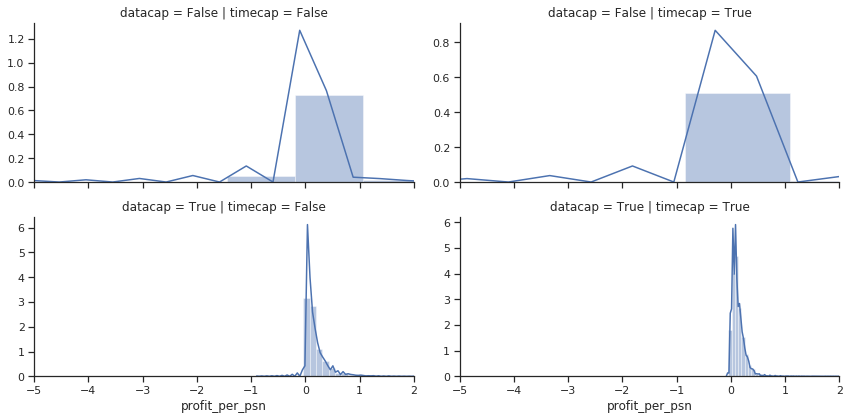
\includegraphics[width=\textwidth,height=2.60417in]{figures/profit_dist.png}
\caption{Distribution of profit}
\end{figure}

\hypertarget{missing-data-and-imputation}{%
\paragraph{Missing data and
imputation}\label{missing-data-and-imputation}}

In general, the data set did not suffering from missing data greatly.
The most critical feature that has missing data is
\texttt{total\ passengers}. Without this information, we cannot generate
our model target and this must be imputed. We chose to impute with those
sessions with the median of that airline and aircraft type.

Also, close to 0.1\% of flights indicate that there were more passengers
than seats available, which is nonsensical. In these cases we replace
the value with the median number of passengers for that aircraft type.

For night flights, which is a categorical feature for which roughly 10\%
are missing, we also impute by defaulting to false. For international
flight, of which approximately 3\% are of unknown status, we impute by
examining the origin and destination countries.

For all boolean features describing amenities such as in-flight
entertainment, TV available, and assorted luxury items, of which less
than 1\% are missing, we impute by defaulting to false.

\begin{longtable}[]{@{}cc@{}}
\caption{Proportion of missing data}\tabularnewline
\toprule
\endhead
\begin{minipage}[t]{0.48\columnwidth}\centering
\textbf{Total Passengers}\strut
\end{minipage} & \begin{minipage}[t]{0.27\columnwidth}\centering
2.77\%\strut
\end{minipage}\tabularnewline
\begin{minipage}[t]{0.48\columnwidth}\centering
\textbf{Data cap(MB)}\strut
\end{minipage} & \begin{minipage}[t]{0.27\columnwidth}\centering
71.74\%\strut
\end{minipage}\tabularnewline
\begin{minipage}[t]{0.48\columnwidth}\centering
\textbf{Time cap(min)}\strut
\end{minipage} & \begin{minipage}[t]{0.27\columnwidth}\centering
62.07\%\strut
\end{minipage}\tabularnewline
\begin{minipage}[t]{0.48\columnwidth}\centering
\textbf{Flight Type}\strut
\end{minipage} & \begin{minipage}[t]{0.27\columnwidth}\centering
2.77\%\strut
\end{minipage}\tabularnewline
\begin{minipage}[t]{0.48\columnwidth}\centering
\textbf{Night Flight}\strut
\end{minipage} & \begin{minipage}[t]{0.27\columnwidth}\centering
10.59\%\strut
\end{minipage}\tabularnewline
\begin{minipage}[t]{0.48\columnwidth}\centering
\textbf{In flight entertainment}\strut
\end{minipage} & \begin{minipage}[t]{0.27\columnwidth}\centering
0.07\%\strut
\end{minipage}\tabularnewline
\begin{minipage}[t]{0.48\columnwidth}\centering
\textbf{TV}\strut
\end{minipage} & \begin{minipage}[t]{0.27\columnwidth}\centering
0.07\%\strut
\end{minipage}\tabularnewline
\begin{minipage}[t]{0.48\columnwidth}\centering
\textbf{Phone}\strut
\end{minipage} & \begin{minipage}[t]{0.27\columnwidth}\centering
0.07\%\strut
\end{minipage}\tabularnewline
\bottomrule
\end{longtable}

At this point we have a cleaned dataset of flights with identifiable
features and imputed values. Unfortunately, only the proportion of
observations that have data allowance or time allowance are roughly
one-third each. Because they are such important features (see fig. 4),
we decided to model these subsets separately. The three subsets are:

\begin{enumerate}
\def\labelenumi{\arabic{enumi}.}
\tightlist
\item
  Has data cap: indepedent variable includes data cap (mb)
\item
  Has time cap: indepedent variable includes time cap (min)
\item
  Full data set: use the boolean flag of whether the product has cap
\end{enumerate}

\begin{longtable}[]{@{}cccc@{}}
\caption{Proportion of data with data/time allowance}\tabularnewline
\toprule
\begin{minipage}[b]{0.16\columnwidth}\centering
hasDataCap\strut
\end{minipage} & \begin{minipage}[b]{0.16\columnwidth}\centering
hasTimeCap\strut
\end{minipage} & \begin{minipage}[b]{0.12\columnwidth}\centering
n\strut
\end{minipage} & \begin{minipage}[b]{0.16\columnwidth}\centering
percentage\strut
\end{minipage}\tabularnewline
\midrule
\endfirsthead
\toprule
\begin{minipage}[b]{0.16\columnwidth}\centering
hasDataCap\strut
\end{minipage} & \begin{minipage}[b]{0.16\columnwidth}\centering
hasTimeCap\strut
\end{minipage} & \begin{minipage}[b]{0.12\columnwidth}\centering
n\strut
\end{minipage} & \begin{minipage}[b]{0.16\columnwidth}\centering
percentage\strut
\end{minipage}\tabularnewline
\midrule
\endhead
\begin{minipage}[t]{0.16\columnwidth}\centering
0\strut
\end{minipage} & \begin{minipage}[t]{0.16\columnwidth}\centering
0\strut
\end{minipage} & \begin{minipage}[t]{0.12\columnwidth}\centering
1566602\strut
\end{minipage} & \begin{minipage}[t]{0.16\columnwidth}\centering
37.46\%\strut
\end{minipage}\tabularnewline
\begin{minipage}[t]{0.16\columnwidth}\centering
0\strut
\end{minipage} & \begin{minipage}[t]{0.16\columnwidth}\centering
1\strut
\end{minipage} & \begin{minipage}[t]{0.12\columnwidth}\centering
1433085\strut
\end{minipage} & \begin{minipage}[t]{0.16\columnwidth}\centering
34.27\%\strut
\end{minipage}\tabularnewline
\begin{minipage}[t]{0.16\columnwidth}\centering
1\strut
\end{minipage} & \begin{minipage}[t]{0.16\columnwidth}\centering
0\strut
\end{minipage} & \begin{minipage}[t]{0.12\columnwidth}\centering
1029065\strut
\end{minipage} & \begin{minipage}[t]{0.16\columnwidth}\centering
24.61\%\strut
\end{minipage}\tabularnewline
\begin{minipage}[t]{0.16\columnwidth}\centering
1\strut
\end{minipage} & \begin{minipage}[t]{0.16\columnwidth}\centering
1\strut
\end{minipage} & \begin{minipage}[t]{0.12\columnwidth}\centering
152794\strut
\end{minipage} & \begin{minipage}[t]{0.16\columnwidth}\centering
3.65\%\strut
\end{minipage}\tabularnewline
\bottomrule
\end{longtable}

\hypertarget{gradient-boostinglightgbm}{%
\subsection{5. Gradient
Boosting/lightGBM}\label{gradient-boostinglightgbm}}

LightGBM is a gradient boosting framework that uses tree-based learning
algorithm. It was designed for distributed training and it splits the
tree leaf wise with the best fit. The framework is fast and lower memory
usages. The gradient boosting has two primary method: bagging and
boosting. Bagging involves the training of independent models and
combines their prediction. When we want to reduce the variance of
decision tree, we used bagging and random forest is one of the example.
If single model has low performance, bagging will not get a better bias,
but boosting could generate a combined model with lower error. Both are
good at reducing variance and provide higher stability, however, if the
single model is overfitting, bagging would be the best option.

When we consider decision trees, we start with an \(F_0\)(initial fit)
The constant value that minimize the loss function L is:

\[
    F_0(x)=argmin_{\rho}\sum_{i=1}^nL(y_i,\rho)
\] In the case of optimizing the MSE, we take the mean of the target
values \(F_0(x)=\dfrac{1}{n}\sum_{i=1}^ny_i\)

Calculate pseudo residual with initial guess of \(F_0\)

\[
    r_{i1}=-\dfrac{\partial L(y_i,F_{0}(x_i))}{\partial F_{0}(x_i)}
\]

Now, we can fit the decision tree \(h_1(x)\) to the residuals . In order
to minimize the loss for each leaf, we apply gradient descent by
stepping in the direction of average gradient for the leaf nodes from
the decision tree \(h_1(x)\) yielding a new boosted fit of the data:
\(F_1(x)=F_{0}(x)+\lambda_1\rho_1h_1(x)\) where \(\lambda_1\) is
learning rate

\hypertarget{gradient-boosting-algorithm}{%
\paragraph{Gradient Boosting
Algorithm}\label{gradient-boosting-algorithm}}

Let M be a number of boosting rounds and L be a differential loss
function L: \[
    F_0(x)=arg_r min\sum_{i=1}^nL(y_i,\gamma)
\] For m=1 to M

Calculate the pseudo residuals \[
    \overset{\sim}{y_{i}}=-\dfrac{\partial L(y_i,F_{m-1}(x_i))}{\partial F_{m-1}(x_i)}
\] Fit decision tree \(h_m(x)\) to \(\overset{\sim}{y_{i}}\) Compute the
step multiplier \(\rho_m\) for each leaf of \(h_m(x)\) Let
\(F_m(x)=F_{m-1}(x)+\lambda_m\rho_mh_m(x)\) where \(\lambda_m\) is the
learning rate for iteration m.

We chose to use lightGBM for two main reasons:

\begin{enumerate}
\def\labelenumi{\arabic{enumi}.}
\tightlist
\item
  Its ability to handle categorical features directly
\item
  Its performance in computational time and accurarcy
\end{enumerate}

For our problem, we have found that the geographical features provided a
lot of information and wanted to include the country level details. For
instance, if we were to use XGBoost, another high performance gradient
boosting framework, we would need to use one-hot encoding on the
categorical features. With 134 unique originating and destination
countries, there would be 268 encoding columns. In contrast, lightGBM
allowed categorical feature to be label encoded with a much smaller
memory footprint.

\hypertarget{results}{%
\subsection{6. Results}\label{results}}

\hypertarget{training}{%
\paragraph{Training}\label{training}}

Model fitting was done by using 80:20 train/validate split with 5 fold
cross validation.\\
Model parameters were searched using randomized grid search.

\hypertarget{errors}{%
\paragraph{Errors}\label{errors}}

\begin{longtable}[]{@{}lll@{}}
\caption{Proportion of data with data/time allowance}\tabularnewline
\toprule
Subset & Metric & Value\tabularnewline
\midrule
\endfirsthead
\toprule
Subset & Metric & Value\tabularnewline
\midrule
\endhead
Data capped & RMSE & 0.1522\tabularnewline
Data capped & MAE & 0.0838\tabularnewline
Time capped & RMSE & 0.4501\tabularnewline
Time capped & MAE & 0.0839\tabularnewline
Full dataset & RMSE & 0.1551\tabularnewline
Full dataset & MAE & 0.0840\tabularnewline
\bottomrule
\end{longtable}

\hypertarget{feature-importance}{%
\paragraph{Feature importance}\label{feature-importance}}

Feature importance here is calculated by the number of times a feature
is used in a split. We can see that flight duration is on the very top
for all three subsets. This is to be expected, since our model target is
the rate of profit per flight generated by a particular product.
Naturally, any product have more opportunity to generate revenue given
extra exposure.

\pagebreak

\begin{figure}
\centering
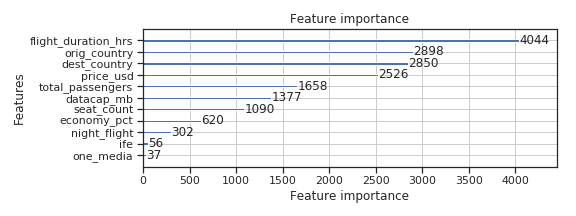
\includegraphics[width=\textwidth,height=2.08333in]{figures/featimp_dc.png}
\caption{Feature importance (data capped subset)}
\end{figure}

\begin{figure}
\centering
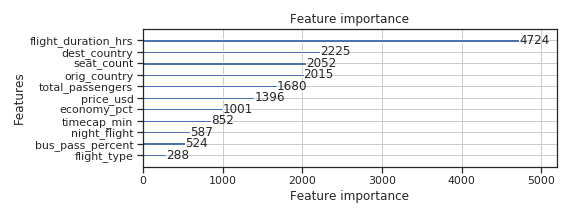
\includegraphics[width=\textwidth,height=2.08333in]{figures/featimp_tc.png}
\caption{Feature importance (time capped subset)}
\end{figure}

\begin{figure}
\centering
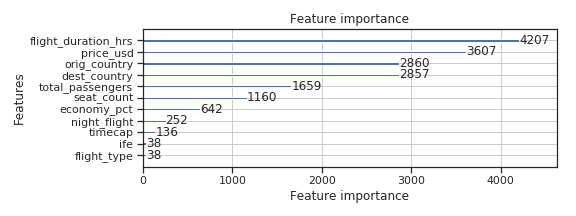
\includegraphics[width=\textwidth,height=2.08333in]{figures/featimp_full.png}
\caption{Feature importance (full dataset)}
\end{figure}

\hypertarget{next-steps}{%
\subsection{Next steps}\label{next-steps}}

We are currently working on using the tuned model to generate pricing
recommendation. For routes with data cap, the pricing policy will
include both price and data allowance. For other routes, the
recommendation will be pricing only.

\pagebreak

\hypertarget{references}{%
\subsection{References}\label{references}}

\begin{itemize}
\tightlist
\item
  Ke, G., Meng, Q., Finley, T., Wang, T., Chen, W., Ma, W., Ye, Q., \&
  Liu, T. (2017). LightGBM: A Highly Efficient Gradient Boosting
  Decision Tree. NIPS.
\item
  Shakya, Kern, Owusu, and Chin. ``Neural Network Demand Models and
  Evolutionary Optimisers for Dynamic Pricing.'' Knowledge-Based Systems
  29 (2012): 44-53. Web.
\item
  Bauer, and Jannach. ``Optimal Pricing in E-commerce Based on Sparse
  and Noisy Data.'' Decision Support Systems 106 (2018): 53-63. Web.
\item
  Owusu, G., Voudouris, Kern, Garyfalos, Anim-Ansah, and Virginas. ``On
  Optimising Resource Planning in BT Plc with FOS.'' 2006 International
  Conference on Service Systems and Service Management 1 (2006): 541-46.
  Web.
\item
  Shakya, Chin, and Owusu. ``An AI-based System for Pricing Diverse
  Products and Services.'' Knowledge-Based Systems 23.4 (2010): 357-62.
  Web.
\item
  Friedman ``Greedy Function Approximation:A Gradient Boosting
  Machine.'' (2001): Web.
\end{itemize}


\end{document}
